\chapter{Introduction}\label{cap:introduction}

This chapter aims to give a general introduction to the research project and put it into wide scientific and societal context.
It defines the main research question and the hypothesis, and gives a high-level overview of the proposed framework.
It also provides the links to the original datasets and the code.

\section{Context}
Forests are a crucial part of the global ecosystem, both environmentally and economically.
They cover a third of the land area, contain over 80\% of terrestrial biodiversity, and somewhere around one-third of humanity depends on forests and forest products for their livelihoods [\citet{aertsForestRestorationBiodiversity2011}; \citet{StateWorldsForests2020}].
Forests are an essential renewable natural resource and a huge, dynamic part of the global carbon cycle.
Figure~\ref{fig-forest-coverage} offers a map of the global tree coverage based on data from \citet{hansenHighResolutionGlobalMaps2013} to highlight the extent of forests on the planet.
Responsible management of forests allows using the resources efficiently and sustainably, preserving the biodiversity, and regulating atmospheric $CO_2$, which is becoming especially important as the anthropogenic climate change is ongoing and accelerating [\citet{faheyForestCarbonStorage2010}; \citet{forsterIndicatorsGlobalClimate2024}].
This drives the need for accurate, detailed, up-to-date information about various forest attributes such as distributions of tree species, average heights and ages of trees, estimates of trunk diameter, timber volume, and above ground biomass, and others.

The traditional manual forest inventories that rely on people going out into the forest to count and measure trees are extremely labor-intensive and time-consuming, which makes them infeasible to cover extensive areas with sufficient detail, speed, and frequency \citep{burleyEncyclopediaForestSciences2004}.
This is especially relevant in countries where massive areas are covered by forests, such as Russia, Brazil, Canada, USA, and China, which are the top five countries for forest area according to \citet{GlobalForestResources2020}.
For that reason, various remote sensing techniques are widely used to extend and extrapolate the traditional forest inventories.
All sorts of data, from satellite and aerial imagery to very detailed terrestrial LiDAR surveys, are used in all sorts of applications that require mapping forest attributes.
Some such applications are mentioned in the next chapter dedicated to reviewing the literature.

\begin{figure}
\centering{
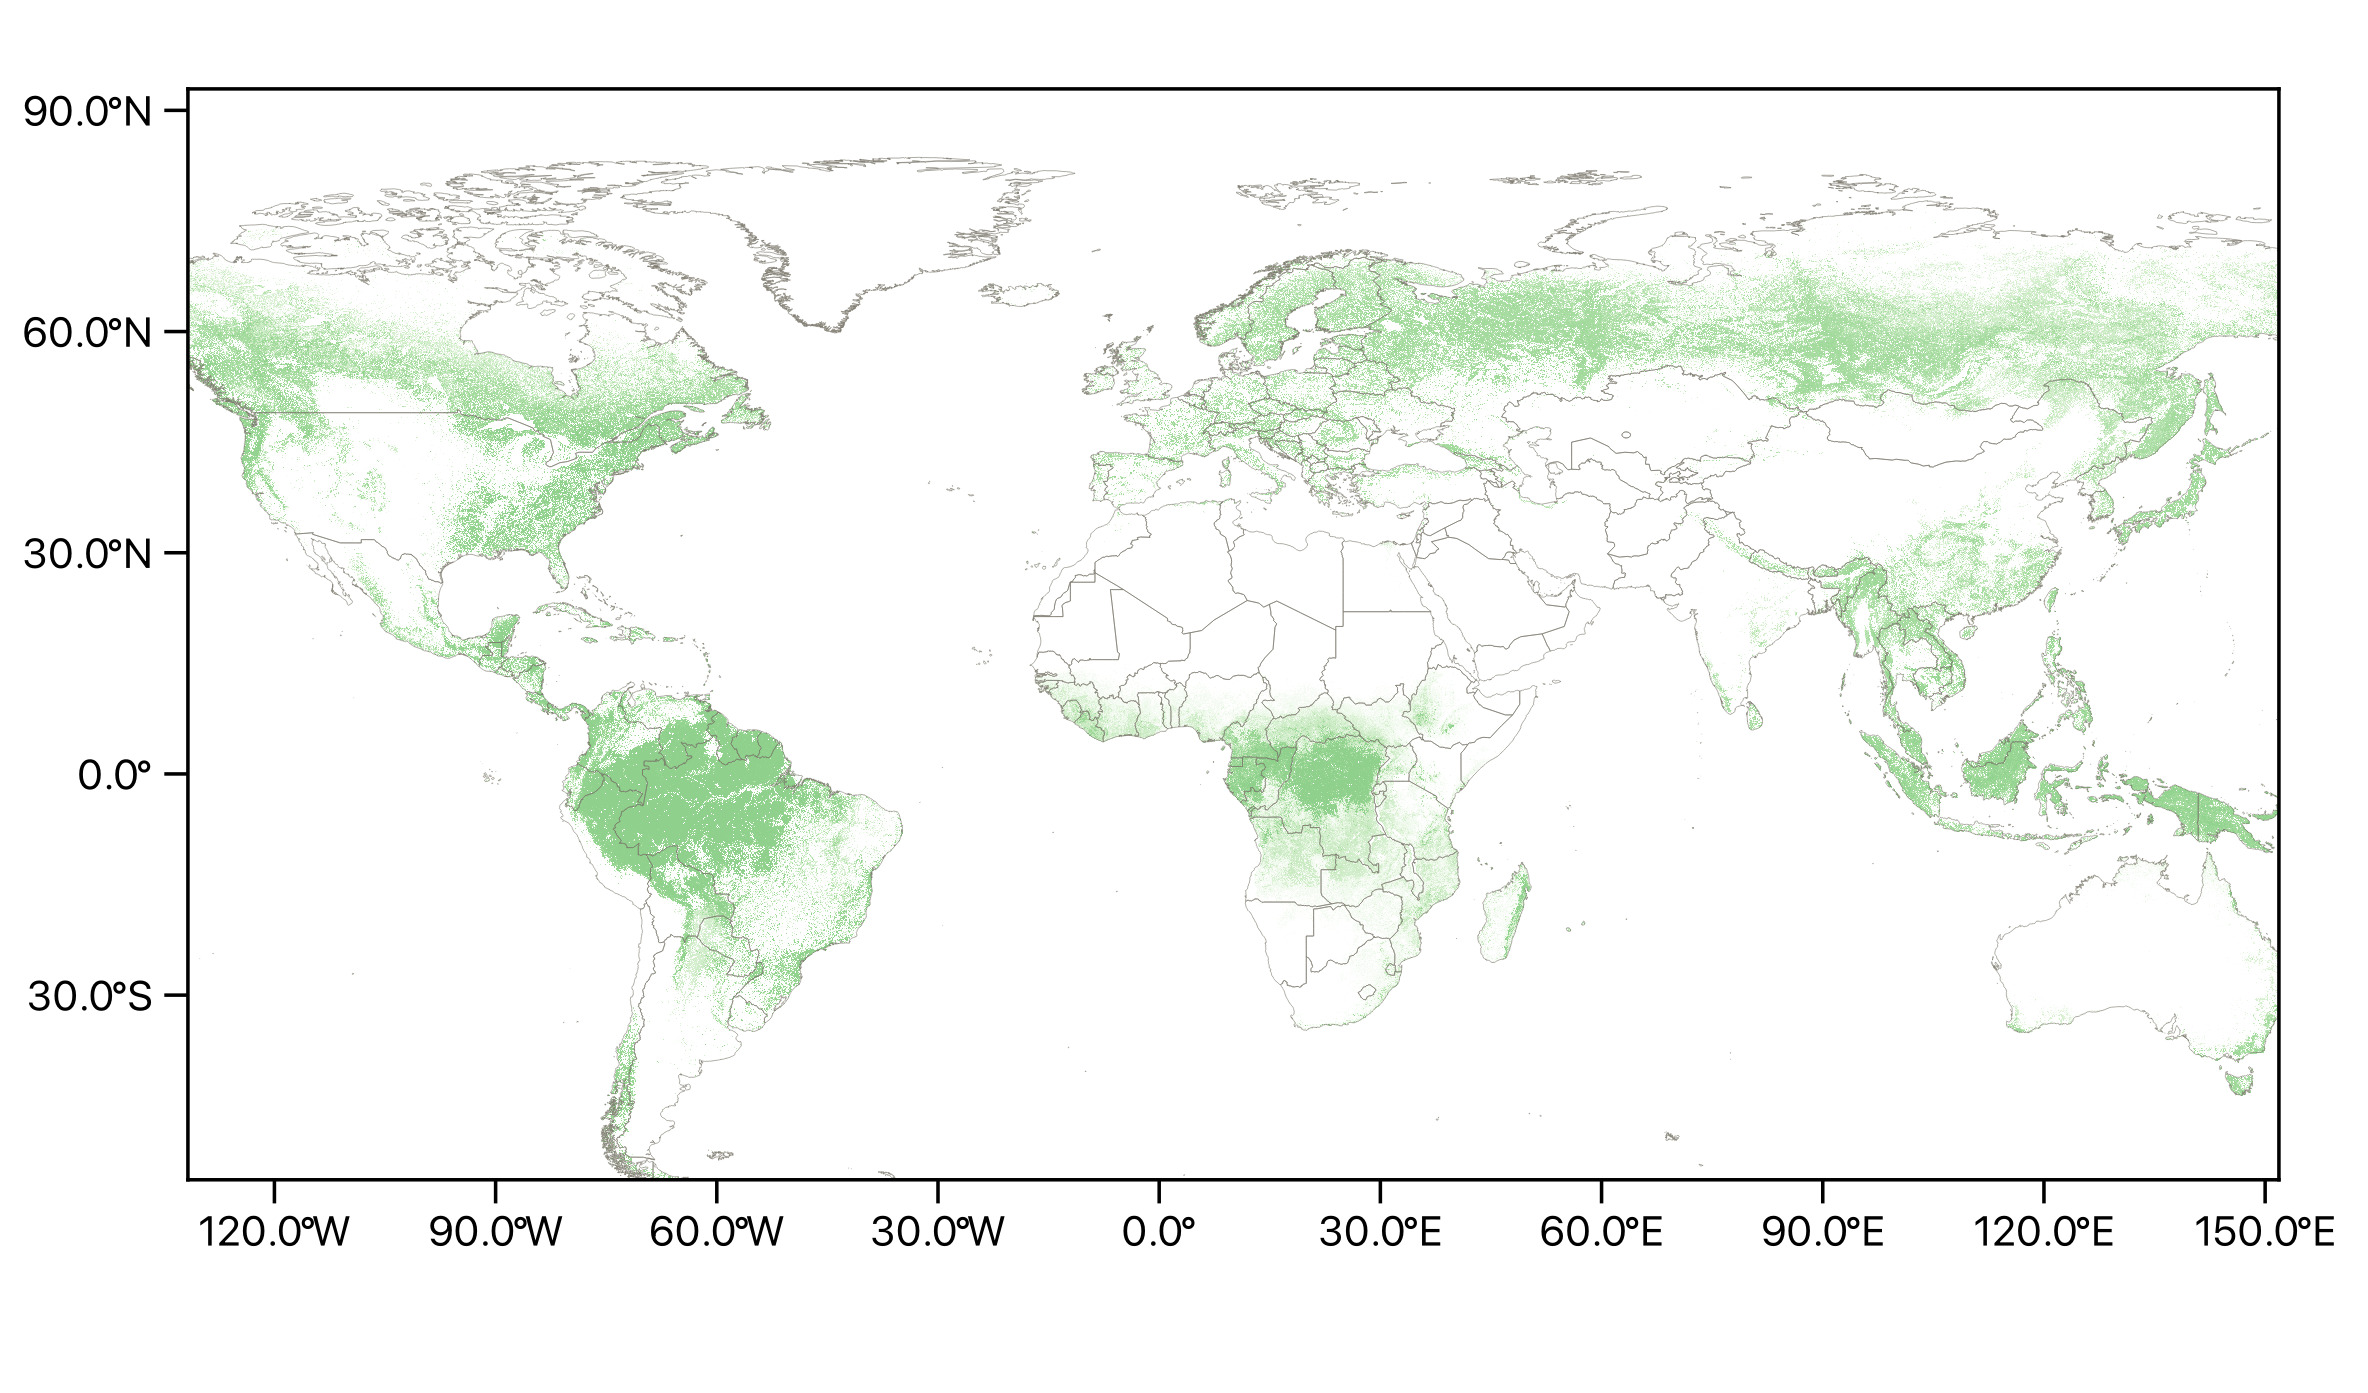
\includegraphics[width=\textwidth]{../images/global-forest-cover.jpg}
}
\caption[Global tree cover map]{\label{fig-forest-coverage}Global tree cover for 2010. Data from \citet{hansenHighResolutionGlobalMaps2013}
}
\end{figure}

Many national space agencies even provide open access to satellite data that can be used for mapping forests.
European Space Agency offers free and open access\footnote{Although the access is not open for everyone equally, as I have observed silent bans of the accounts connecting from Russian IP-addresses without any response to support inquires.} to the Sentinel missions, including C-band SAR data from Sentinel-1 and medium-resolution multispectral data from Sentinel-2, both with global coverage.
They also have an upcoming P-band SAR mission called BIOMASS, designed specifically to study global forest biomass and carbon cycles \citep{queganEuropeanSpaceAgency2019}, which further indicates the growing importance and interest in the topic of forest mapping.
NASA provides free access to an abundance of satellite data through its Earthdata platform, Landsat mission with the Operation Land Imager (OLI) instrument and Terra mission with Moderate Resolution Imaging Spectroradiometer (MODIS) instrument being the most relevant for forest mapping applications.
The Indian Space Research Organisation, Brazilian National Institute for Space Research, National Space Research and Development Agency of Nigeria all offer free satellite data that can be used for this purpose.
NASA and the ISRO also have a joint upcoming mission called NISAR with two fully-polarimetric SAR sensors at L-band and S-band \citep{kelloggNASAISROSyntheticAperture2020}, which will benefit forestry applications greatly.

The open satellite data is an essential tool for wide-area studies, but it usually has coarse resolution, which limits the achievable accuracy and level of detail.
It also offers no ability to control the observation parameters, as they are fixed by the instrument configuration and orbit parameters, both of which are outside the data consumer control.
Higher resolution data with a limited ability to control the acquisition parameters is available commercially, but the prices are steep.
Aerial observations with sensors mounted on planes or helicopters are both more controllable and cheaper alternatives, although still expensive and sill limited in the flexibility of the control of acquisition parameters.
A much more affordable and controllable alternative is UAV-based observation.
It allows for fine-grained control and on the fly adjustment of many important parameters such as flight height, flight path overlap, combination of used sensors, and so on.

The most common way to use UAV remote sensing, be it LiDAR, multispectral, hyperspectral, or other data modalities, for mapping forest attributes in industry is what is known in the LiDAR community as the area-based approach, described in detail in Section~\ref{sec-area-based-approach}.
It is based on extrapolating measurements from ground plots made in traditional inventories by aggregating remote sensing data to the grid with cell area of a ground plot, which results in coarse resolution maps.
It is easy to use, but its results are often not detailed enough when working on smaller scales.
However, modern sensors and processing techniques allow not aggregating at all and instead working on the level of individual trees, which is as detailed as it can possibly get, allowing for any level of aggregation for downstream tasks.
This requires robust algorithms that allow detecting individual trees in dense multimodal data.
This is relatively\footnote{The word relatively does a lot of heavy lifting here, as the problem is by no means easy on its own and takes a lot of effort from many researchers to continue to make progress on.
} easy in urban environments, manually planted and managed forest stands, or forests that are either sparse or predominantly coniferous, where the structure of the canopy is easy to interpret.
In some such environments, state-of-the-art results can be achieved by simple local maxima detection algorithms, that rely on the assumption that a tree can be detected by finding peaks on of canopies because they correspond to tree tops.
Forest that are mixed and dense, which are a huge part of forests in countries mentioned earlier, are much harder to work with and are a very active area of research for developing methods of detection of individual trees.
The canopies in such forests are very complex, especially because the top of the crowns of deciduous tree species often don't have a single pronounced height maximum, and crowns of nearby trees often overlap.

The framework described in this thesis focuses on fusion of two remote sensing data sources, UAV LiDAR point clouds and UAV RGB orthophotos, to detect individual trees in dense mixed forests and predict required attributes for each tree individually, producing the most detailed maps possible.
The choice of data sources is driven by their complementary nature, which I believe is key for semantically parsing such complex environments.
LiDAR is an active sensor, which means it does not depend on external conditions such as lightning.
Cloud and terrain shadows, incidence angles, and weather conditions do not affect LiDAR surveys.
Moreover, LiDAR provides 3D vertical structural information about the forest, as laser pulses penetrate the canopy and reach both the undergrowth and the ground.
This structural information is essential for understanding complex environments like dense forests.
High-resolution RGB imagery does depend on the lighting, but is still an invaluable tool, as it offers detailed data with fixed resolution, continuous coverage of surfaces, unlike the discrete representation of laser scanning, and captures many fine details and textures.
It can also benefit from a huge variety of well-established tools and processing techniques from the field of computer vision.
Neither of these data sources on their own is enough to reliably and with sufficient robustness separate individual trees in dense mixed forests, and the key to success lies in their fusion.

\section{Research question and hypothesis}\label{sec-research-question}

The main research question could be formulated as follows: "How to reduce effort and cost required for detailed inventories of dense mixed forests without losing accuracy?"
The main hypothesis is then: "An accurate and detailed inventory with reduced effort and cost can be achieved through fusion of UAV LiDAR and RGB data using machine learning".
The benchmarks to measure against are both the traditional manual forest inventory and the widely used area-based approach.

Cost and effort are closely connected, as any effort is in the end converted to cost.
Still, it often makes sense to separate the two to highlight the nature of the effects the proposed system should have.
The cost reduction was partly addressed in the previous section during the discussion of the platform of choice: UAV-based remote sensing offers a great balance of upfront cost, effort to operate, and versatility in observation parameters.
The effort reduction comes from greatly decreasing the amount of field inventory data required when using the proposed system, from the relative ease of collection of remote sensing data compared to alternatives, and from relative ease of tuning the system to operate in new areas.

\section{Overview of the framework}

The proposed framework described in this thesis consist of a neural-network based tree segmentation in UAV LiDAR point clouds enhanced with RGB orthophoto-based features and processing the segments with a collection of specialized classic machine learning models that predict the parameters of interest for each detected tree.
The tree segmentation model is trained on synthetic forest patches constructed from a dataset of point clouds of individual trees extracted manually from a large UAV LiDAR survey, heavily relying on augmentations to make the synthetic forest closer to real forest.
The parameter prediction classification and regression models are trained on the same dataset of individual trees using a collection of widely used manual point cloud features.
Figure~\ref{fig-framework-apply} is a schematic representation of the framework, showing the required inputs in red, processing steps in yellow, and artifacts in cyan.
The field inventory is phased out, but it is still required, as application of any framework requires quality assessment and validation.

\begin{figure}
\centering{
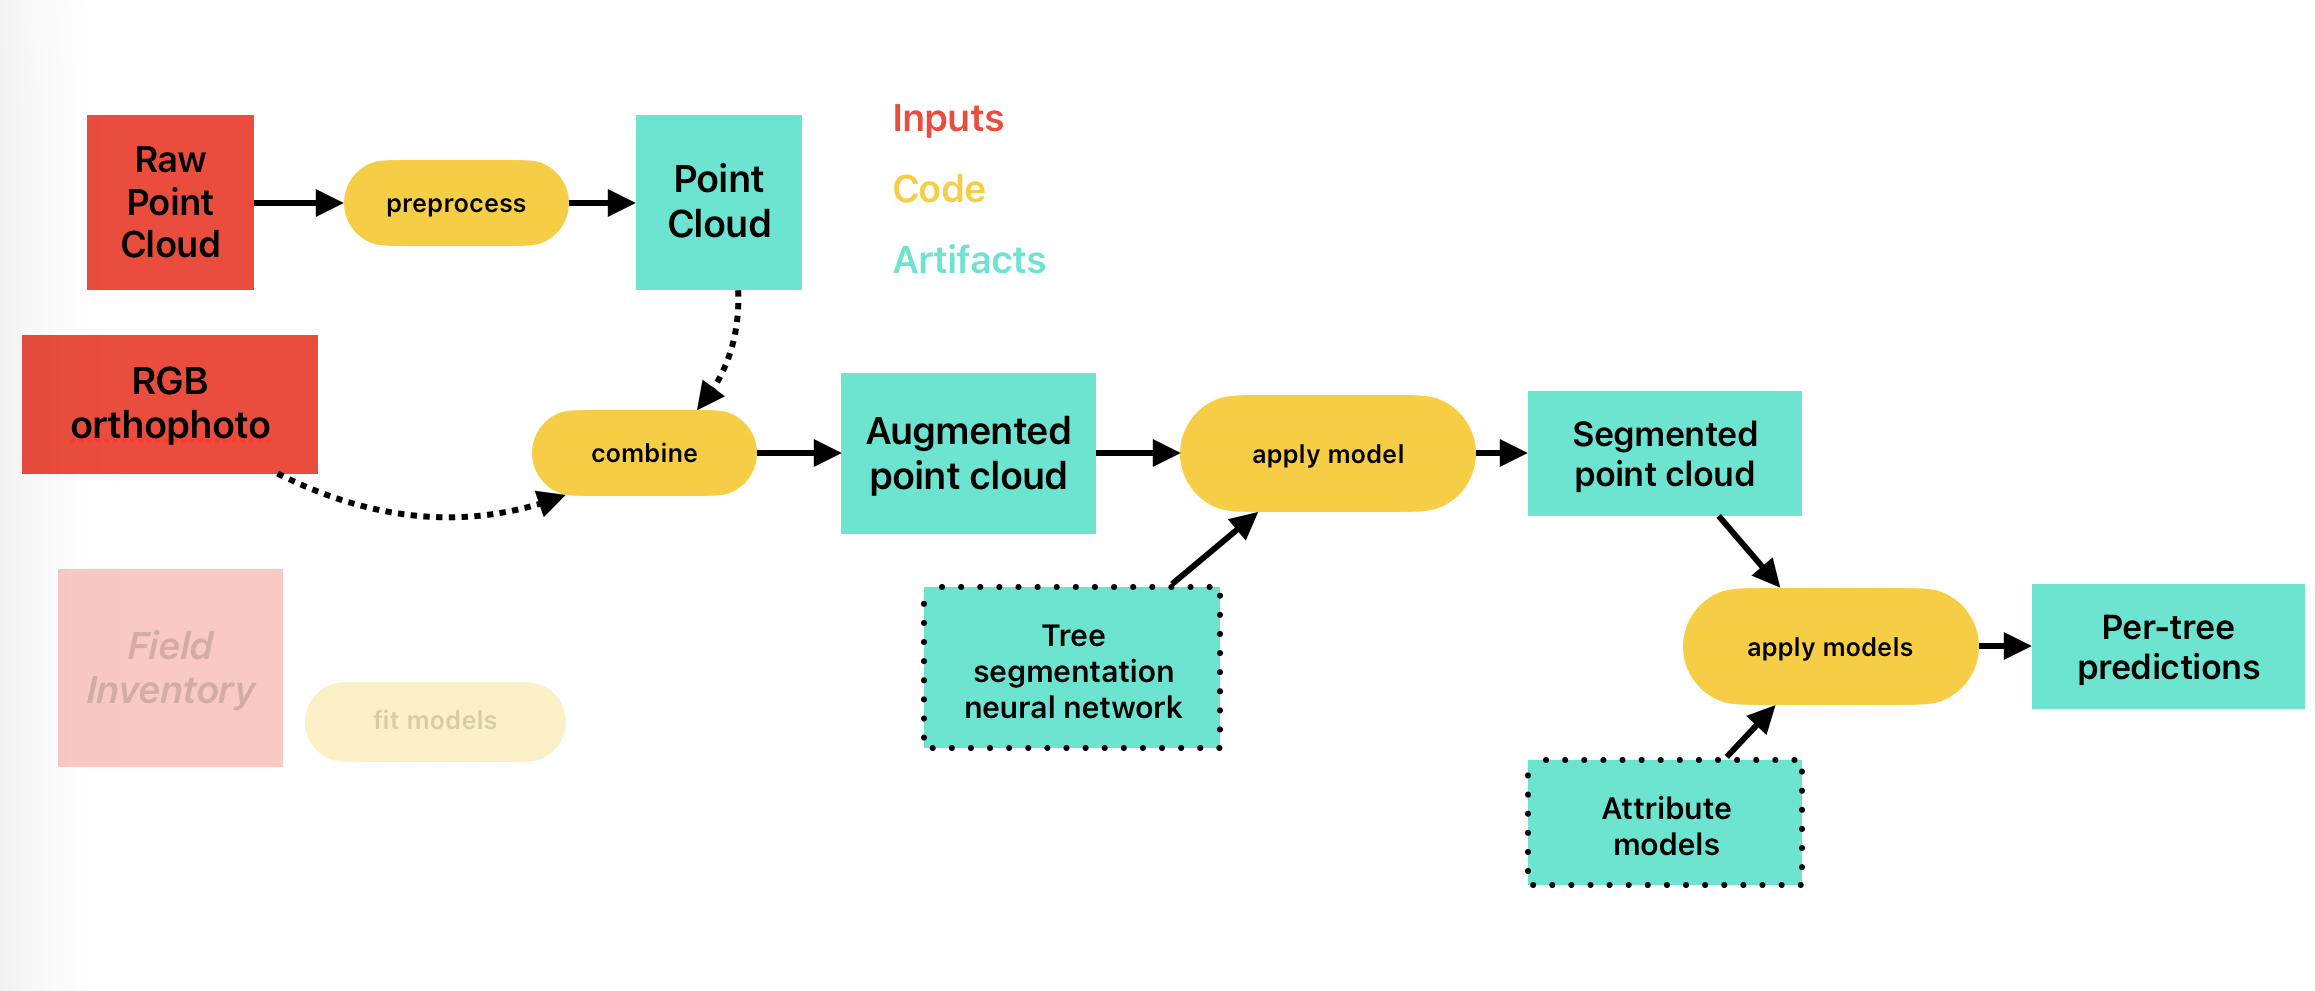
\includegraphics[width=\textwidth]{../images/framework_application_schematic.jpg}
}
\caption[Schematic representation of the framework: application]{\label{fig-framework-apply}The schematic representation of the
framework in the application stage.}
\end{figure}

Figure~\ref{fig-framework-prepare} is a schematic of the preparation step for the framework.
Each individual node is described in detail in Section~\ref{sec-materials-and-methods}.


\begin{figure}
\centering{
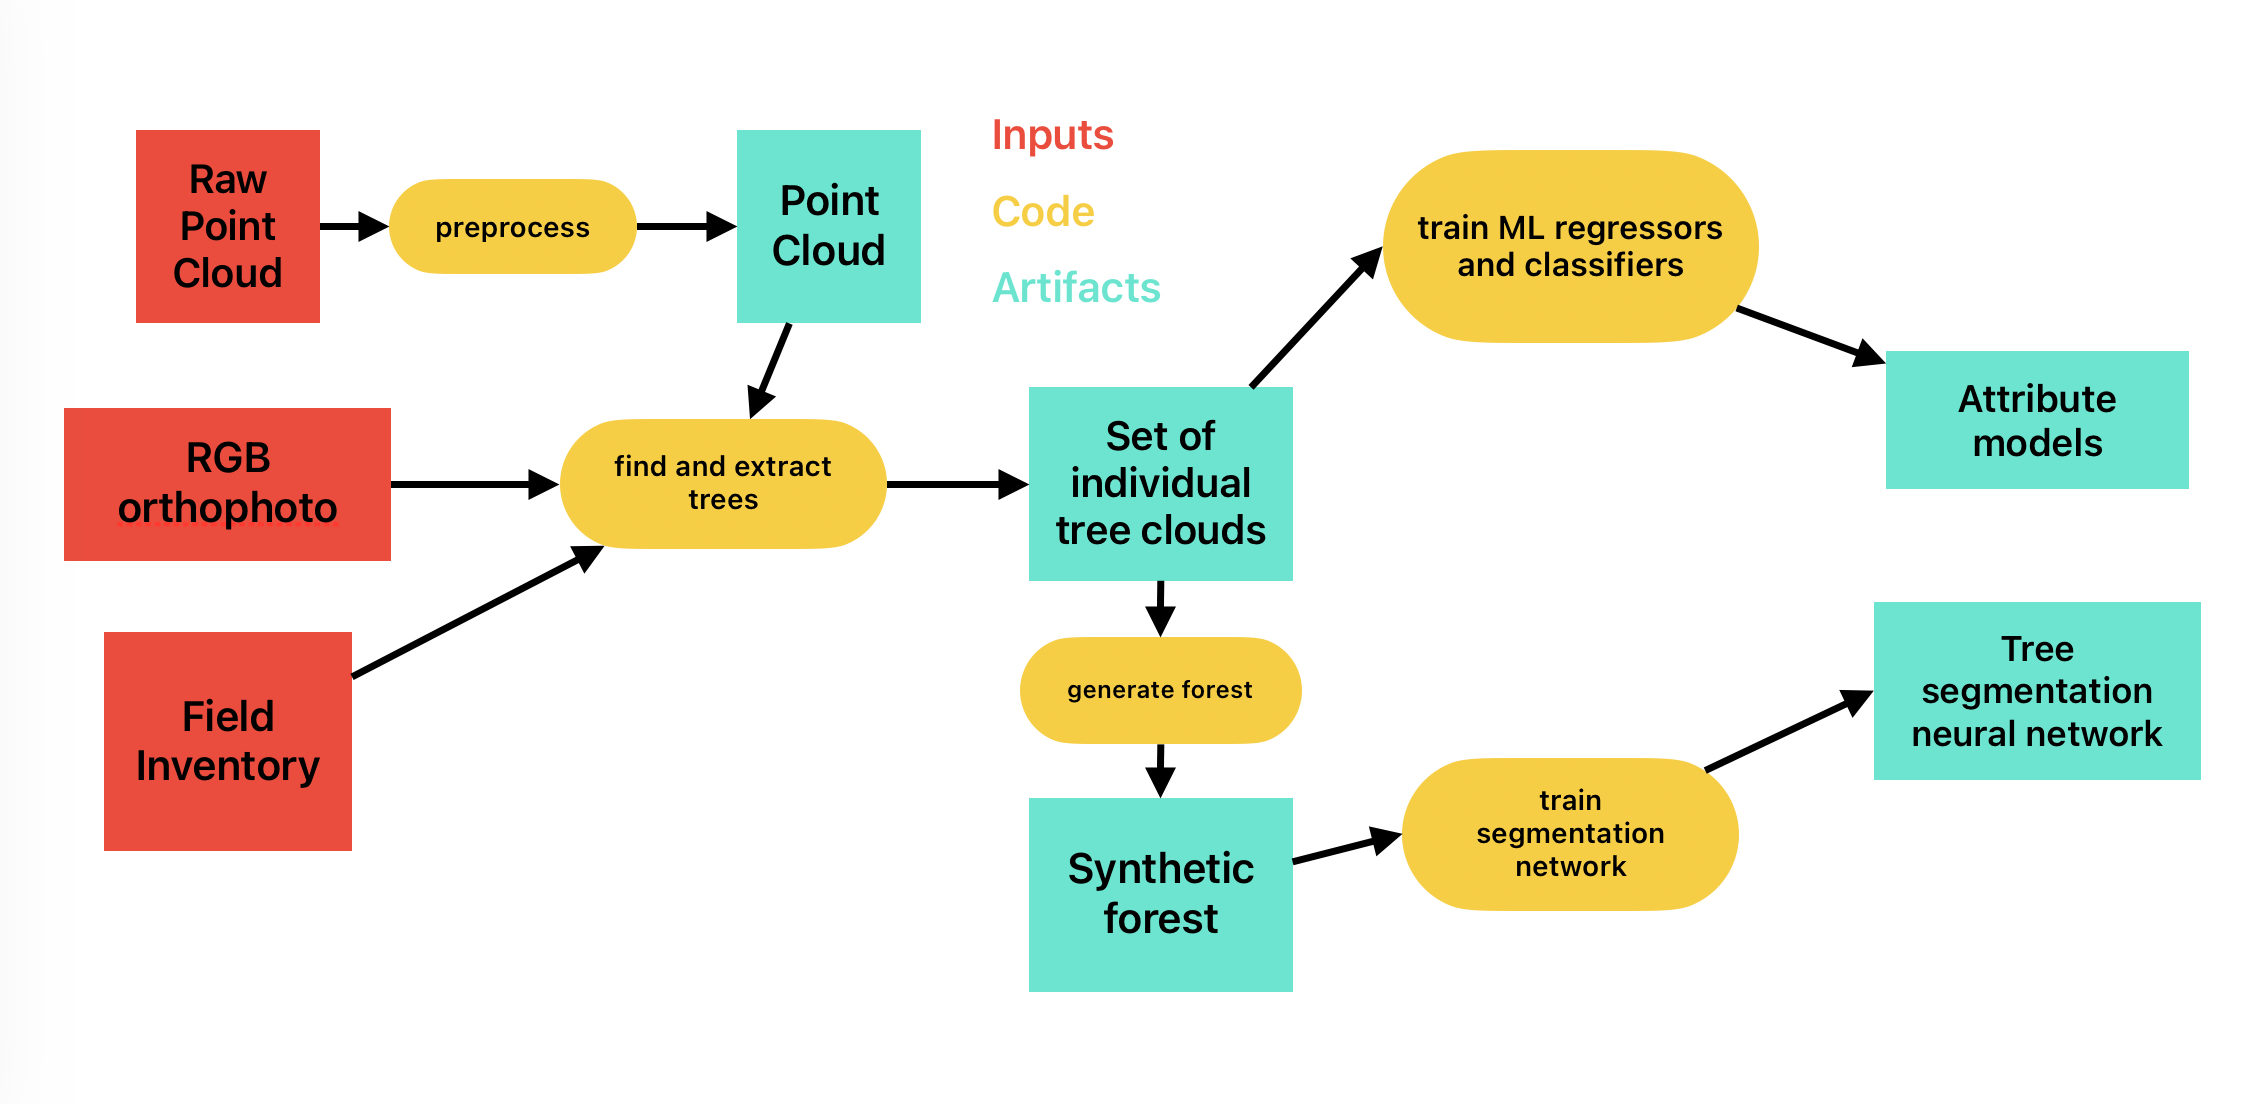
\includegraphics[width=\textwidth]{../images/framework_preparation_schematic.jpg}
}
\caption[Schematic representation of the framework: preparation]{\label{fig-framework-prepare}The schematic representation of
the framework in the preparation stage.}
\end{figure}

\section{Thesis Structure}

\begin{description}
    \item[\Autoref{cap:introduction} - Introduction]
The Introduction chapter aims to give a general introduction to the research project and put it into wide scientific and societal context.
It defines the main research question and the hypothesis, and gives a high-level overview of the proposed framework.
It also provides the links to the original datasets and the code.

    \item[\Autoref{cap:literature} - Literature Review]
The Literature Review chapter aims to give an overview of the scientific literature on topics most relevant to the project.
Its main goals are to provide the reader with context for the research described in the thesis, provide references for in-depth materials on topics that are out of scope of this work, and to highlight the research gap that the work tries to address.

	\item[\Autoref{cap:materials} - Materials and methods]
The Materials and Methods chapter describes in detail the datasets, methods and methodological choices used in the proposed framework.
Its aim is to make the work reproducible and to explain the methodological choices made.

	\item[\Autoref{cap:results} - Results]
The Results chapter describes the results of each stage of the framework preparation and the validation approach used to verify its applicability and effectiveness on realistic data.

    \item[\Autoref{cap:conclusion} - Conclusion]
The Conclusion chapter offers a brief summary of the thesis as a whole, potential perspectives for further improvement of the proposed framework, and some concluding thoughts.

\end{description}

\section{Data and code availability}

Original datasets described in the thesis are openly available on Kaggle \href{https://www.kaggle.com/datasets/sentinel3734/tree-detection-lidar-rgb}{here} and \href{https://www.kaggle.com/datasets/sentinel3734/uav-point-clouds-of-individual-trees}{here}.
All the code used for the project is available on GitHub at \href{https://github.com/iod-ine/phd}{iod-ine/phd}.
An HTML version of this thesis is hosted through GitHub Pages and is available \href{https://iod-ine.github.io/thesis}{here}.
The thesis document was developed using Quarto \cite{Allaire_Quarto_2024} using the literate programming approach \cite{knuth84}, and a link to an HTML version hosted through GitHub Pages is available in the repository.
The deep learning part is implemented using PyTorch \cite{Ansel_PyTorch_2_Faster_2024}, PyTorch Geometric \cite{Fey_Fast_Graph_Representation_2019}, and PyTorch Lightning \cite{Falcon_PyTorch_Lightning_2019}, with experiment tracking using MLflow.
Classic machine learning models implementations are from scikit-learn \cite{scikit-learn}.
NumPy \cite{2020NumPy-Array}, SciPy \cite{2020SciPy-NMeth}, pandas \cite{The_pandas_development_team_pandas-dev_pandas_Pandas}, scikit-image \cite{van_der_Walt_scikit-image_image_processing_2014} libraries are used for processing the data.
ratserio \cite{gillies_2019}, geopandas, laspy, lazrs libraries are used for working with geospatial data formats.
matplotlib \cite{Hunter_Matplotlib_A_2D_2007} and seaborn \cite{waskomSeabornStatisticalData2021} libraries are used for visualization.
